\section{Complex Valued Functions}
Denote the association of the \textbf{value} $f(z)$ to $z$ as:
\[z \mapsto f(z) \]

\begin{defn}[\textbf{Complex Valued Function}]
	\[f(z) = u(z) +iv(z)\]
	\[f(z) = f(x + iy) = u(x,y) + iv(x,y)\]
	\[z \mapsto u(z) \;\; \text{and} \;\;  z \mapsto v(z) \]
\end{defn}

So a complex valued function can be represented as functions of $2$ \textit{real variables.}

Example:
\begin{align*}
	f(z) &= (x - iy)^2 \\
	&= (x - iy)(x - iy) \\
	\\
	\therefore \; f(z) &= x^2 - y^2 - i2xy
\end{align*}
With $u$ and $v$ given by:
\begin{align*}
	u(z) &= u(x, y) = x^2 - y^2 \\
	v(z) &= v(x, y) = -2xy \\
	\\
	\therefore \; f(z) &= u(x, y) + iv(x, y) \\
	&= u(z) + iv(z) \\
\end{align*}

\subsection{Power Function}
The most important example of complex valued functions.
\begin{defn}[\textbf{Power Function}]
Any function of the form:
	\[f(z) = z^n\]
\end{defn}

\subsection{Polar coordinates}
Write $z$ in polar coordinates using $|z| = r \in \mathbb{R}$ and $\theta \in [0, 2\pi]$.

\begin{defn}[\textbf{Complex Numbers and Functions in Polar Form}]
	\begin{align*}
		z &= re^{i\theta} \;\;\;\;\;\; = \cos{\theta} + i\sin{\theta} \\
		f(z) &= r^ne^{in\theta} \;\; = r^n(\cos{n\theta} + i\sin{n\theta}) \\
	\end{align*}
\end{defn}


\subsection{Closed/Open Disc}
\begin{defn}[\textbf{Set of the Closed Disc} $\overline{D}$]
	\begin{align*}
		\overline{D} = &\{z \in \mathbb{C} \;\;|\;\; \forall z \leq 1 \} \\
		\\
		\forall z \in \overline{D}&, \; n \in \mathbb{N}: \;\;\; z \mapsto z^n \in \overline{D} \\
	\end{align*}
\end{defn}

The \textbf{Open Disc} changes $z < 1.$

\subsection{Unit Disc / Roots of Unity}

\textbf{Intent:} Break the unit circle up into $n$ sectors/tiles/slices.

\textbf{Motivation:} Allows mapping solutions for polynomials, which themselves represent complex numbers or 
analytic functions, to roots of unity over $[0, 2\pi].$

\begin{defn}[\textbf{Sector of Unit Circle}]
	\begin{align*}
		S = \left\{ z \in \mathbb{C} \;\; | \;\; z = e^{i\theta} ,\;\;\;  0 \leq \theta \leq \frac{2\pi}{n} \right\} \\
	\end{align*}
\end{defn}

\subsubsection*{Function of a Real Variable}
Suppose $r \in \mathbb{R}$ with a function defined by:
\[r \mapsto r^n \]
This maps the unit interval $[0, 1]$ onto itself:
\[[0, 1] \to [0, 1] \]

\subsubsection*{Function of Theta}
Suppose $\theta \in [0, 2\pi]$ with a function defined by:
\[\theta \mapsto n\theta \]
This maps the interval $[0, \frac{2\pi}{n}]$ onto the circumference of a circle $[0, 2\pi]$:
\[ \left[ 0, \frac{2\pi}{n} \right] \to [0, 2\pi] \]

\subsubsection*{Function of a Complex Value}
Combining above the function $f(z) = z^n$ maps the sector $S$ onto the full disc of numbers $w$ where:

\[w = te^{i\varphi} \]
\[0 \leq t \leq 1\]
\[0 \leq \varphi \leq 2\pi \]

Things to note:
\begin{itemize}
	\item The power function tiles the unit disc $D_1$ by sector $S$ a total of $n$ times. 
	\item So $z \mapsto z^n$ wraps the disc $n$ times around.
\end{itemize}

Diagram of this tiling for a few factors of $\pi$ with $\theta = 0, \pi/6, \pi/4, \pi/3, \pi/2$:

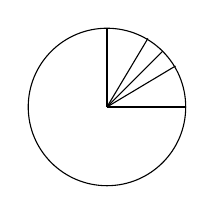
\begin{tikzpicture}
	\draw (0, 0) circle (1cm);
	\draw (0, 0) -- (1,0);
	\draw (0, 0) -- (0.87, 0.52);
	\draw (0, 0) -- (0.71, 0.71);
	\draw (0, 0) -- (0.52, 0.87);
	\draw (0, 0) -- (0, 1);
\end{tikzpicture}

This gives $4$ seperate choices of tile to then multiply by $n$ to cover the unit disc.

To express every complex number $w^n = z$ one ends up with the following generalization:
\begin{defn}[\textbf{Root of Unity}]
	\[\zeta^k = e^{\sfrac{2\pi ik}{n}}\]
\end{defn}
Which has the $n$th power given as:
\[ (\zeta^k)^n = ( e^{\sfrac{2\pi ik}{n}} )^n = e^{2\pi ik} = 1 \]
The points $w_k$ are just the product of $e^{\frac{i\theta}{n}}$ with all the $n$-th roots of unity:
\[w_k = e^{\sfrac{i\theta}{n}}\zeta^k\]

One of the \textbf{major results of the theory of complex variables} is to reduce the study of certain functions, including most of the 
common functions like exponentials, logarithms, sine, cosine; to power series, which can be approximated by polynomials.

Thus the power function is in some sense the unique basic function out of which the others are constructed.
\newpage